\section{PRESENT}

\begin{frame}{PRESENT}
\begin{itemize}
    \item Ultra-lightweight block cipher and has a substitution permutation network.
    \pause
    \item Block length of 64 bits and 80 and 128-bit key sizes.
\end{itemize}
\begin{figure}[h!]
    \centering
    \includegraphics[width=\linewidth]{present/PRESENT_diagram.pdf}
    \caption{SP network for PRESENT cipher \cite{presentdiagram}\footfullcite{presentdiagram}}
    \label{fig:spp}
\end{figure}
\end{frame}
\begin{frame}{Cipher Design}
    \tikzset{
    block/.style = {
        draw, 
        fill=white, 
        rectangle, 
        minimum height=1.8em, 
        minimum width = 10em
    },
    block2/.style = {
        draw, 
        fill=white, 
        rectangle, 
        minimum height=3.7em, 
        minimum width=6em
    },
    sum/.style = {
        draw, 
        fill=white, 
        circle, 
        inner sep=0pt,
        minimum size = 0.5cm
    },
    pinstyle/.style = {
        pin edge={to-,thin,black}
    }
}

\begin{columns}
    \begin{column}{0.5\textwidth}
       \begin{block}{Psuedo-code}
           \begin{algorithmic}
            \STATE{generateRoundKeys()}
            \FOR{$i=1$ \TO $31$ }
                \STATE {addRoundKey(\textsc{State},$K_i$)} 
                \STATE {sBoxLayer(\textsc{State})} 
                \STATE {pLayer(\textsc{State})} 
            \ENDFOR
            \STATE addRoundKey(\textsc{State},$K_{32}$)
        \end{algorithmic}
       \end{block}
    \end{column}
    \begin{column}{0.5\textwidth}  %%<--- here
        \begin{center}
         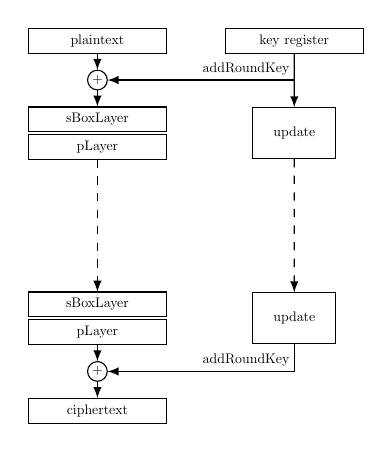
\begin{tikzpicture}[auto, node distance=2cm,>=latex,scale=0.6, every node/.style={scale=0.5}]
            % nodes
            \node [sum] (sum1) {+};
            \node [block,above of=sum1,node distance=1cm] (plaintext) {plaintext};
            \node [block,right of=plaintext,node distance=5cm] (keyregister) {key register};
            \node [block,below of=sum1,node distance=1cm] (sBoxLayer) {sBoxLayer};
            \node [block,below of=sBoxLayer,node distance=0.7cm] (pLayer) {pLayer};
            \node [block,below of=pLayer,node distance=4cm] (sBoxLayer2) {sBoxLayer};
            \node [block,below of=sBoxLayer2,node distance=0.7cm] (pLayer2) {pLayer};
            \node [sum, below of=pLayer2,node distance=1cm] (sum2) {+};
            \node [block,below of=sum2,node distance=1cm] (ciphertext) {ciphertext};
            
            \node [block2,below of=keyregister,node distance=2.35cm] (update) {update};
            \node [block2,below of=update,node distance=4.7cm] (update2) {update};
        
            % arrows
            \draw [->] (plaintext) -- (sum1);
            \draw [->] (sum1) -- (sBoxLayer);
            \draw [->] (pLayer2) -- (sum2);
            \draw [->] (sum2) -- (ciphertext);
            \draw [->] (keyregister) -- (update);
            \draw [->,dashed] (update) -- (update2);
            \draw [->,dashed] (pLayer) -- (sBoxLayer2);
            \draw [->] (keyregister)  |- node[above left= 0pt] {addRoundKey            }    (sum1);
            \draw [->] (update2) |- node[above left= 0pt]{addRoundKey            }   (sum2);
        \end{tikzpicture}
         \end{center}
    \end{column}
    \end{columns}
\end{frame}
\begin{frame}{Key schedule Algorithm}
     We discuss the 80-bit key schedule algorithm.
     \\
     \hspace{40pt}
    \scalebox{0.65}{
    \begin{figure}

        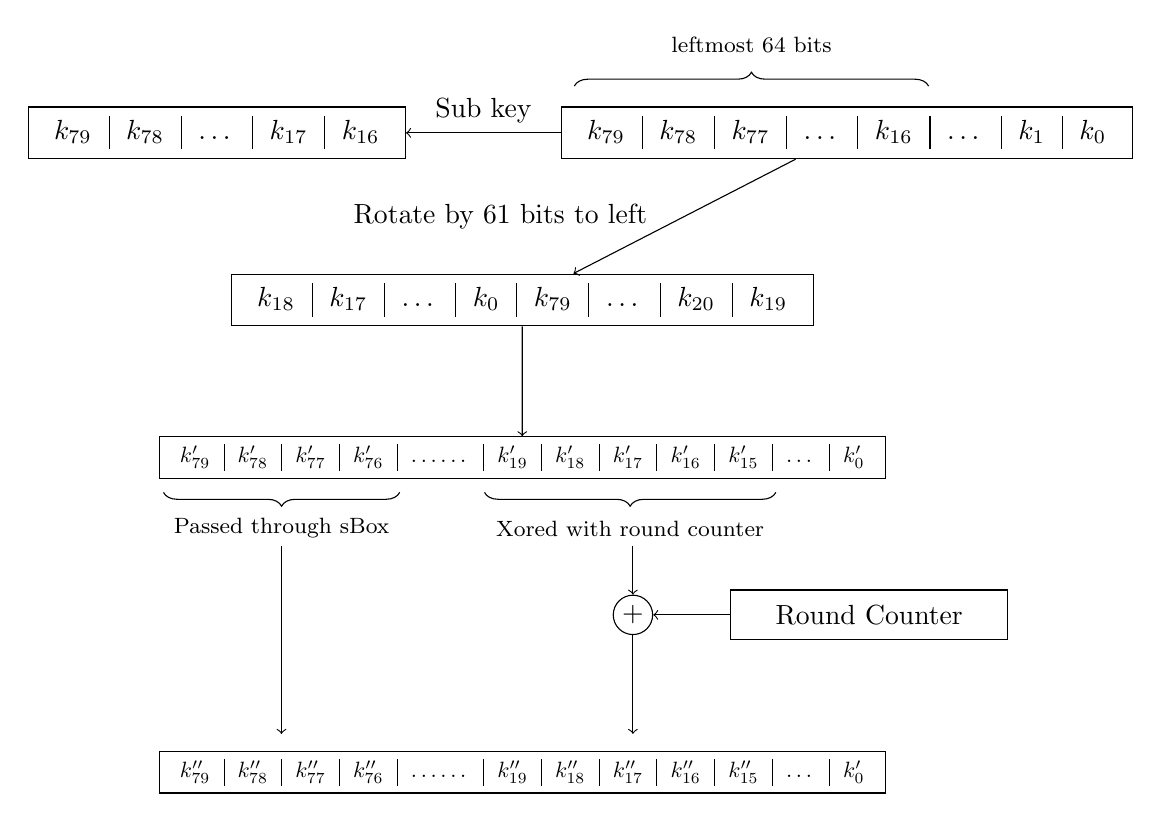
\begin{tikzpicture}
            % nodes
            
            \node (masterkey) [shape = rectangle,draw] {
                \begin{tabular}{c|c|c|c|c|c|c|c}
                    $k_{79}$&$k_{78}$&$k_{77}$&\dots&$k_{16}$&\dots&$k_1$&$k_0$
                \end{tabular}
            };
            \node (subkey) [left of = masterkey,node distance=8cm, shape = rectangle,draw] {
                \begin{tabular}{c|c|c|c|c}
                    $k_{79}$&$k_{78}$&\dots&$k_{17}$&$k_{16}$
                \end{tabular}
            };
            \node (shiftedkey) [below left of =  masterkey,node distance=1cm,shape = rectangle,draw,node distance = 3cm,xshift = -2cm] {
                \begin{tabular}{c|c|c|c|c|c|c|c}
                    $k_{18}$&$k_{17}$&\dots&$k_{0}$&$k_{79}$&\dots&$k_{20}$&$k_{19}$
                \end{tabular}
            };
            \node (shiftedkey2) [below of =  shiftedkey,shape = rectangle,draw,node distance = 2cm,scale = 0.8] {
                \begin{tabular}{c|c|c|c|c|c|c|c|c|c|c|c}
                    $k_{79}'$&$k_{78}'$&$k_{77}'$&$k_{76}'$&\dots\dots&$k_{19}'$&$k_{18}'$&$k_{17}'$&$k_{16}'$&$k_{15}'$&\dots&$k_{0}'$
                \end{tabular}
            };
            
            \node(xor) [sum,below of = shiftedkey2,xshift = 40pt,node distance = 2cm ] {+};
            \node [block,right of=xor,node distance=3cm] (roundCounter) {Round Counter};
            \node (final) [below of =  shiftedkey2,node distance=4cm,shape = rectangle,draw,scale = 0.8] {
                \begin{tabular}{c|c|c|c|c|c|c|c|c|c|c|c}
                    $k_{79}''$&$k_{78}''$&$k_{77}''$&$k_{76}''$&\dots\dots&$k_{19}''$&$k_{18}''$&$k_{17}''$&$k_{16}''$&$k_{15}''$&\dots&$k_{0}'$
                \end{tabular}
            };
            \node (temp1) [below of= shiftedkey2,xshift = -87] {};
            \node (temp2) [below of= shiftedkey2,xshift = -87,yshift = -75] {};
            \node (temp3) [below of= shiftedkey2,xshift = 40] {};
            \node (temp4) [below of= shiftedkey2,xshift = 40,yshift = -75] {};
            
             % arrows
             \draw [decorate,decoration={brace,amplitude=5pt},xshift=-70pt,yshift=-40pt,rotate=180]
             (1,-2) -- (-3.5,-2) node [black,midway,yshift= 15pt] 
             {\footnotesize leftmost 64 bits};
            
             \draw [decorate,decoration={brace,amplitude=5pt},xshift=-190pt,yshift=-73pt]
                (1,-2) -- (-2,-2) node [black,midway,yshift= -13pt] 
                {\footnotesize Passed through sBox};
                
            \draw [decorate,decoration={brace,amplitude=5pt},xshift=-74pt,yshift=-73pt]
            (1.7,-2) -- (-2,-2) node [black,midway,yshift= -13pt] {\footnotesize Xored with round counter};
            
            \draw [->] (masterkey) -- node[above= 0pt]{Sub key}(subkey)  ;
            \draw [->] (masterkey) -- node[left= 10pt]{Rotate by 61 bits to left} (shiftedkey);
            \draw [->] (shiftedkey) -- (shiftedkey2);
            \draw [->] (temp1) -- (temp2);
            \draw [->] (temp3) -- (xor);
            \draw [->] (roundCounter) -- (xor);
            \draw [->] (xor) -- (temp4);
            
             % \draw (nodeXj') -- (nodeD');
        \end{tikzpicture}
    \end{figure}
    }
\end{frame}